\documentclass[11pt,a4paper]{article}
\usepackage{amsmath}
\usepackage{amssymb}
\usepackage{booktabs}
\usepackage{longtable}
\usepackage{geometry}
\geometry{margin=1in}
\usepackage{hyperref}
\usepackage{enumitem}
\usepackage{graphicx}
\usepackage{siunitx}

\title{Engineering Calculation Report: Problem 2-1: Find Resultant Force}
\date{October 14, 2025}

\begin{document}
\maketitle

\section*{Description}
\noindent
\begin{minipage}{\textwidth}
Test law of cosines display with force angles
\end{minipage}
\par

\section{Known Variables}

\begin{longtable}{lSS}
\toprule
Symbol & {Magnitude (unit)} & {Angle ($^\circ$)} \\
\midrule
\endhead
$F1$ & 700\,\text{N} & 60 \\
$F2$ & 450\,\text{N} & 105 \\
\bottomrule
\end{longtable}

\section{Unknown Variables (To Calculate)}

\begin{longtable}{lll}
\toprule
Symbol & Magnitude (unit) & Angle ($^\circ$) \\
\midrule
\endhead
$FR$ & ? & ? \\
\bottomrule
\end{longtable}

\section{Equations Used}

\begin{enumerate}
\item $\Large FR^{2} = F1^{2} + F2^{2} - 2 \cdot F1 \cdot F2 \cdot \cos{180^\circ - (\theta_{}{F2} - \theta_{}{F1}})$
\item $\Large \frac{\sin{alpha}}{F1} = \frac{\sin{gamma}}{FR}$
\end{enumerate}

\section{Step-by-Step Solution}

\begin{enumerate}[label=\textbf{Step \arabic*:},leftmargin=2cm]
\item \textbf{Solve for $FR Magnitude$}

\begin{description}[leftmargin=2cm]
\item[\textbf{Equation:}] \mbox{}

\begin{flalign*}
\Large FR^{2} = F1^{2} + F2^{2} - 2 \cdot F1 \cdot F2 \cdot \cos{180^\circ - (\theta_{}{F2} - \theta_{}{F1}}) &&
\end{flalign*}

\item[\textbf{Substitution:}] \mbox{}

\begin{flalign*}
\Large FR^{2} = (700.00\,\text{N})^{2} + (450.00\,\text{N})^{2} - 2  \cdot  (700.00\,\text{N})  \cdot  (450.00\,\text{N})  \cdot  \cos{135.0^\circ} &&
\end{flalign*}

\item[\textbf{Result:}] \mbox{}

\begin{flalign*}
\Large FR Magnitude = 1066.76\,N &&
\end{flalign*}

\end{description}

\item \textbf{Solve for $FR Direction$}

\begin{description}[leftmargin=2cm]
\item[\textbf{Equation:}] \mbox{}

\begin{flalign*}
\Large \frac{\sin{alpha}}{F1} = \frac{\sin{gamma}}{FR} &&
\end{flalign*}

\item[\textbf{Substitution:}] \mbox{}

\begin{flalign*}
\Large \frac{\sin{alpha}}{700.00\,\text{N}} = \frac{\sin{135.0^\circ}}{1066.76\,\text{N}} &&
\end{flalign*}

\item[\textbf{Result:}] \mbox{}

\begin{flalign*}
\Large FR Direction = 77.35\,^\circ &&
\end{flalign*}

\end{description}

\end{enumerate}


\section{Summary of Results}

\begin{longtable}{llSl}
\toprule
Variable & Name & {Final Value} & Unit \\
\midrule
\endhead
$F1_{x}$ & F1 X-Component & 350 & N \\
$F1_{y}$ & F1 Y-Component & 606.218 & N \\
$F2_{x}$ & F2 X-Component & -116.469 & N \\
$F2_{y}$ & F2 Y-Component & 434.667 & N \\
$FR_{mag}$ & FR Magnitude & 1066.76 & N \\
$FR_{angle}$ & FR Direction & 1.35009 & ° \\
$FR_{x}$ & FR X-Component & 233.531 & N \\
$FR_{y}$ & FR Y-Component & 1040.88 & N \\
\bottomrule
\end{longtable}

\section{Vector Diagram}

\begin{center}
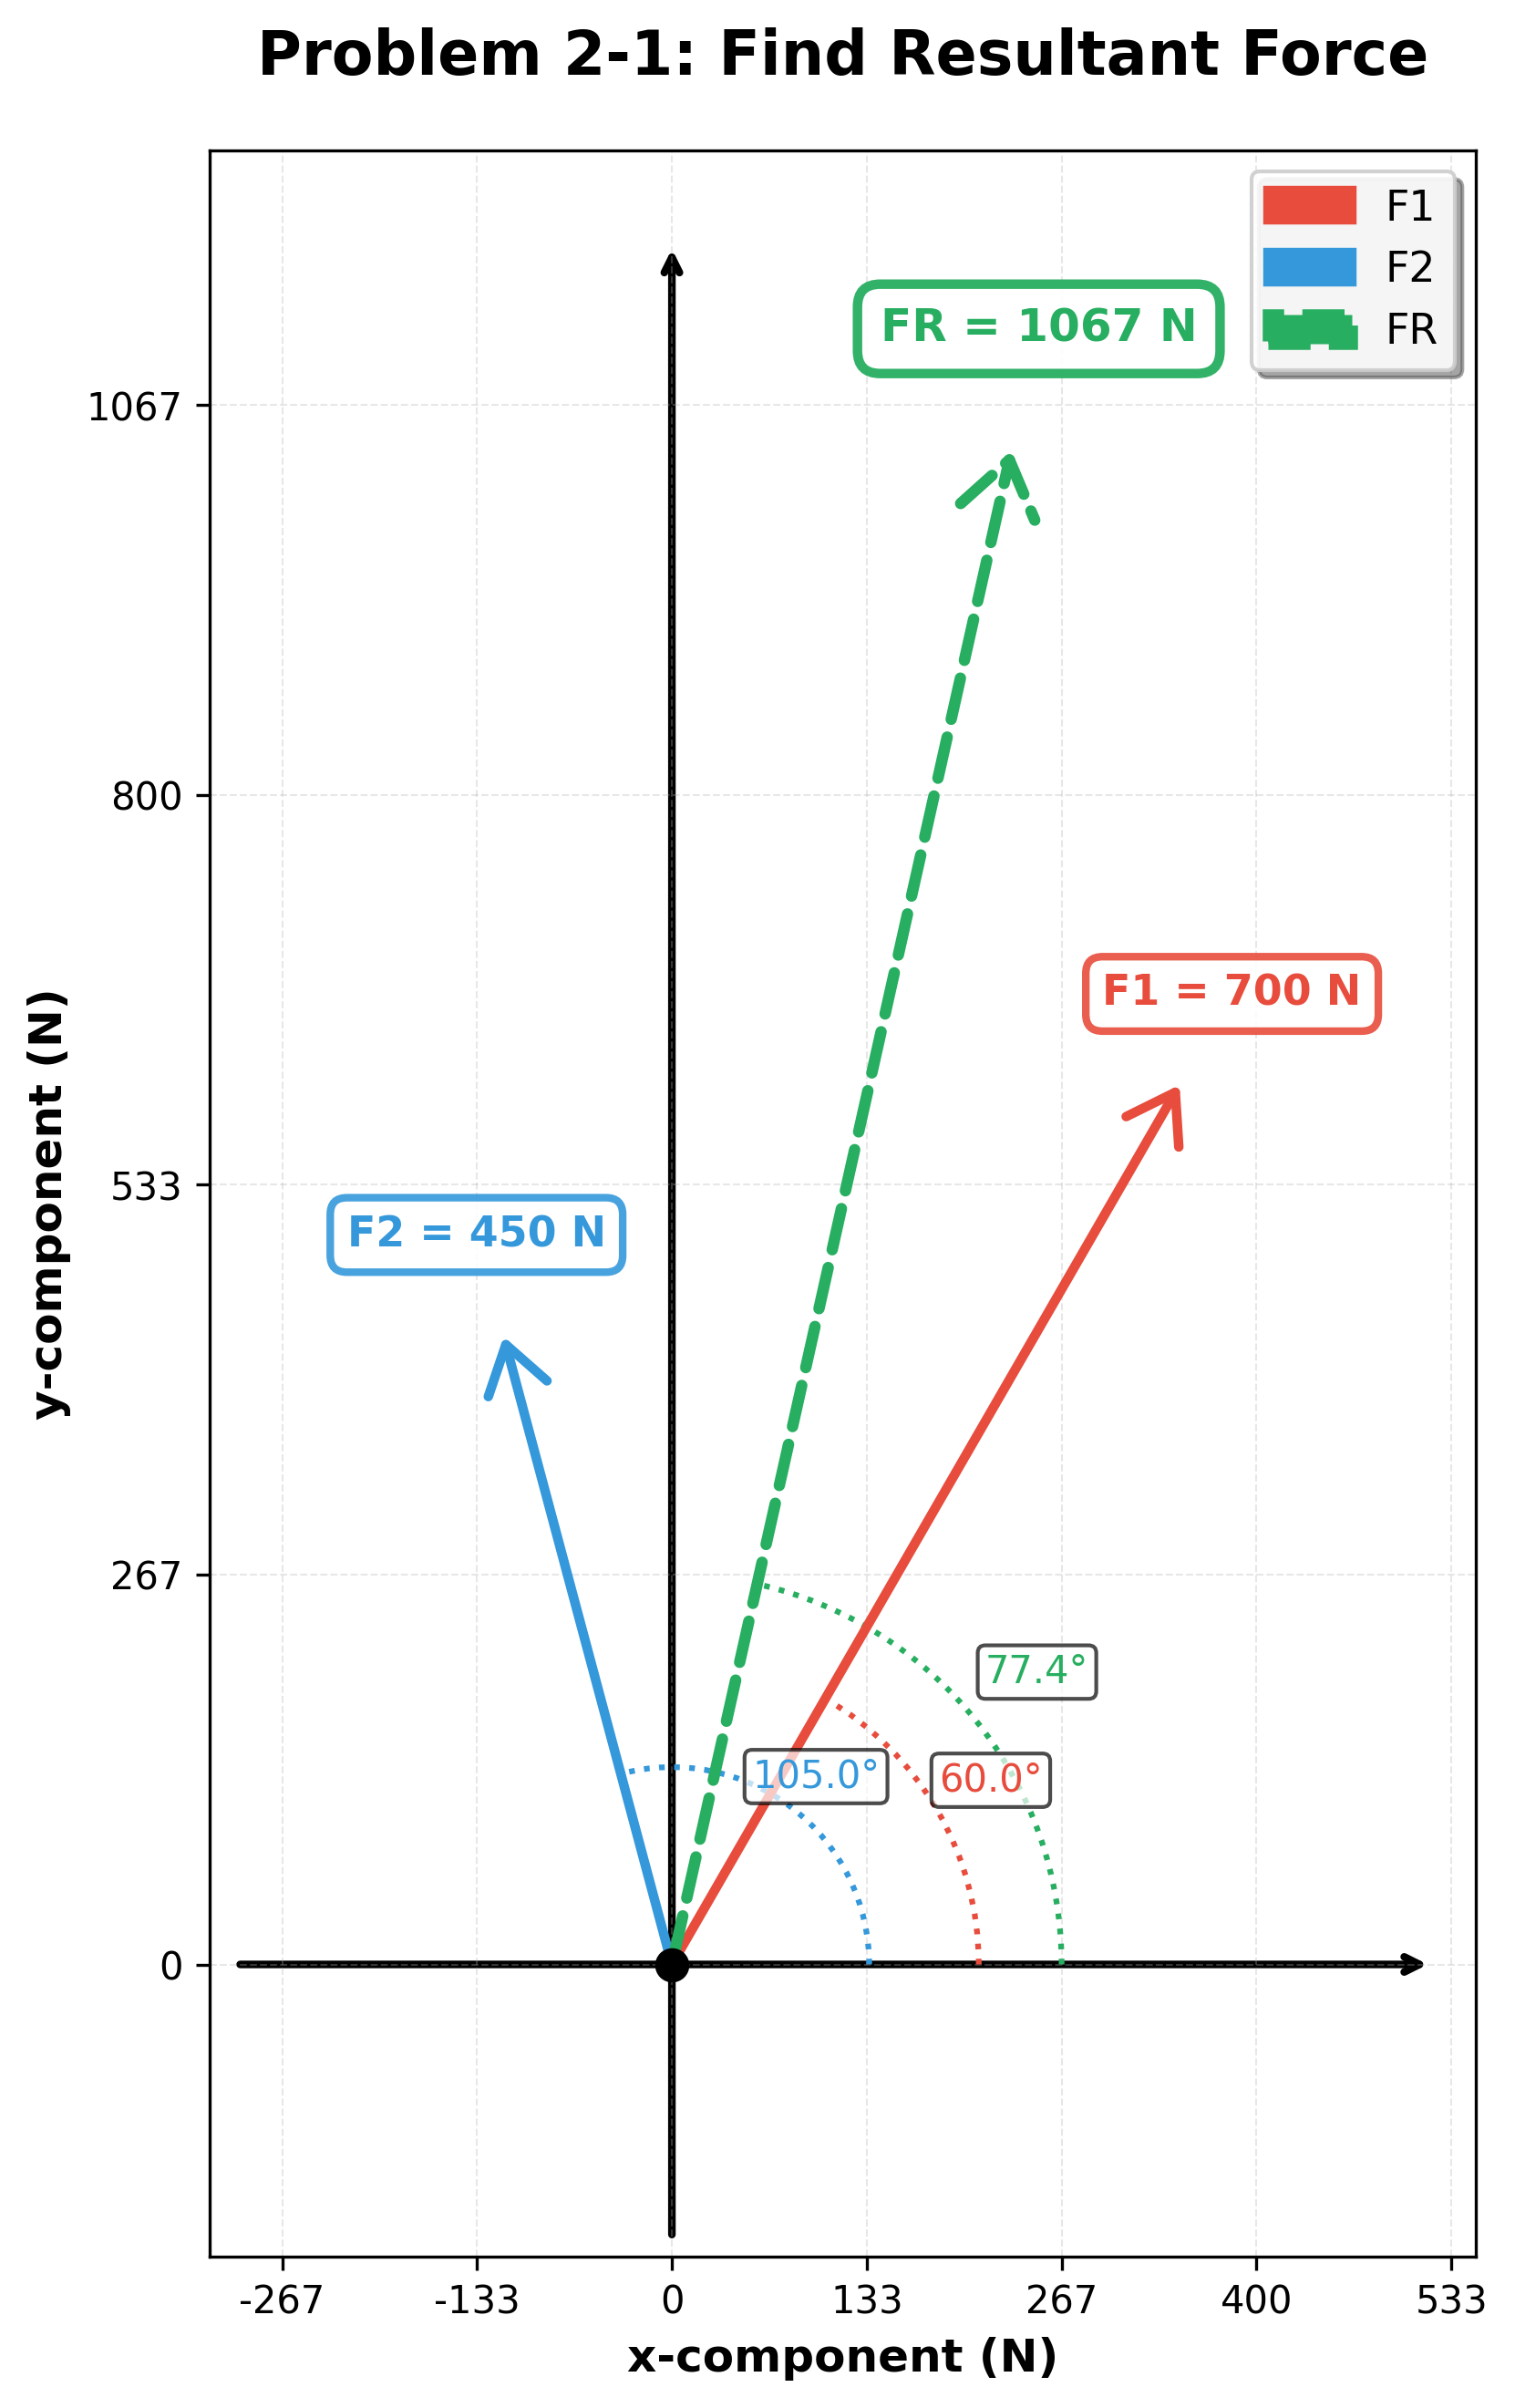
\includegraphics[width=0.7\textwidth]{Problem_2-1_Find_Resultant_Force_diagram.png}
\end{center}

\begin{center}
\textit{Figure: Vector diagram showing all forces and their orientations}
\end{center}


\clearpage

\section*{Disclaimer}
\addcontentsline{toc}{section}{Disclaimer}

\begin{center}
\rule{\textwidth}{0.4pt}
\end{center}

\noindent\textbf{IMPORTANT NOTICE:}

\noindent While every effort has been made to ensure the accuracy and reliability of the calculations provided, we do not guarantee that the information is complete, up-to-date, or suitable for any specific purpose. Users must independently verify the results and assume full responsibility for any decisions or actions taken based on its output. Use of this calculator is entirely at your own risk, and we expressly disclaim any liability for errors or omissions in the information provided.

\vspace{1em}

\noindent\textbf{Report Details:}
\begin{itemize}
\item \textbf{Generated Date:} October 14, 2025
\item \textbf{Generated Using:} Qnty Library
\item \textbf{Version:} Beta (Independent verification required for production use)
\end{itemize}

\vspace{2em}

\noindent\textbf{Professional Review and Approval:}

\vspace{1em}

\begin{longtable}{|p{3cm}|p{4cm}|p{4cm}|p{2.5cm}|}
\hline
\textbf{Role} & \textbf{Name} & \textbf{Signature} & \textbf{Date} \\
\hline
\hline
Calculated By & \rule{0pt}{1.5cm} & & \\
\hline
Reviewed By & \rule{0pt}{1.5cm} & & \\
\hline
Approved By & \rule{0pt}{1.5cm} & & \\
\hline
\end{longtable}

\vspace{1em}

\begin{center}
\rule{\textwidth}{0.4pt}
\vspace{0.5em}
\textit{Report generated using Qnty Library}
\vspace{0.5em}
{\footnotesize For questions or support, please refer to the Qnty documentation}
\end{center}

\end{document}